% Figure 3 composite (vector). Build: pdflatex fig3_assemble.tex
% Identification-first order: row1 define+detect | row2 identification | row3 determinants
\documentclass[tikz,border=1mm]{standalone}
\usepackage{graphicx}\usepackage{helvet}\renewcommand{\familydefault}{\sfdefault}
\begin{document}
\begin{tikzpicture}[x=1mm,y=1mm]
  \useasboundingbox (0,0) rectangle (183,167);
  % row 1: a schematic | b windows | c detection ratio (hero)
  \node[anchor=north west,inner sep=0] at (4,163)  {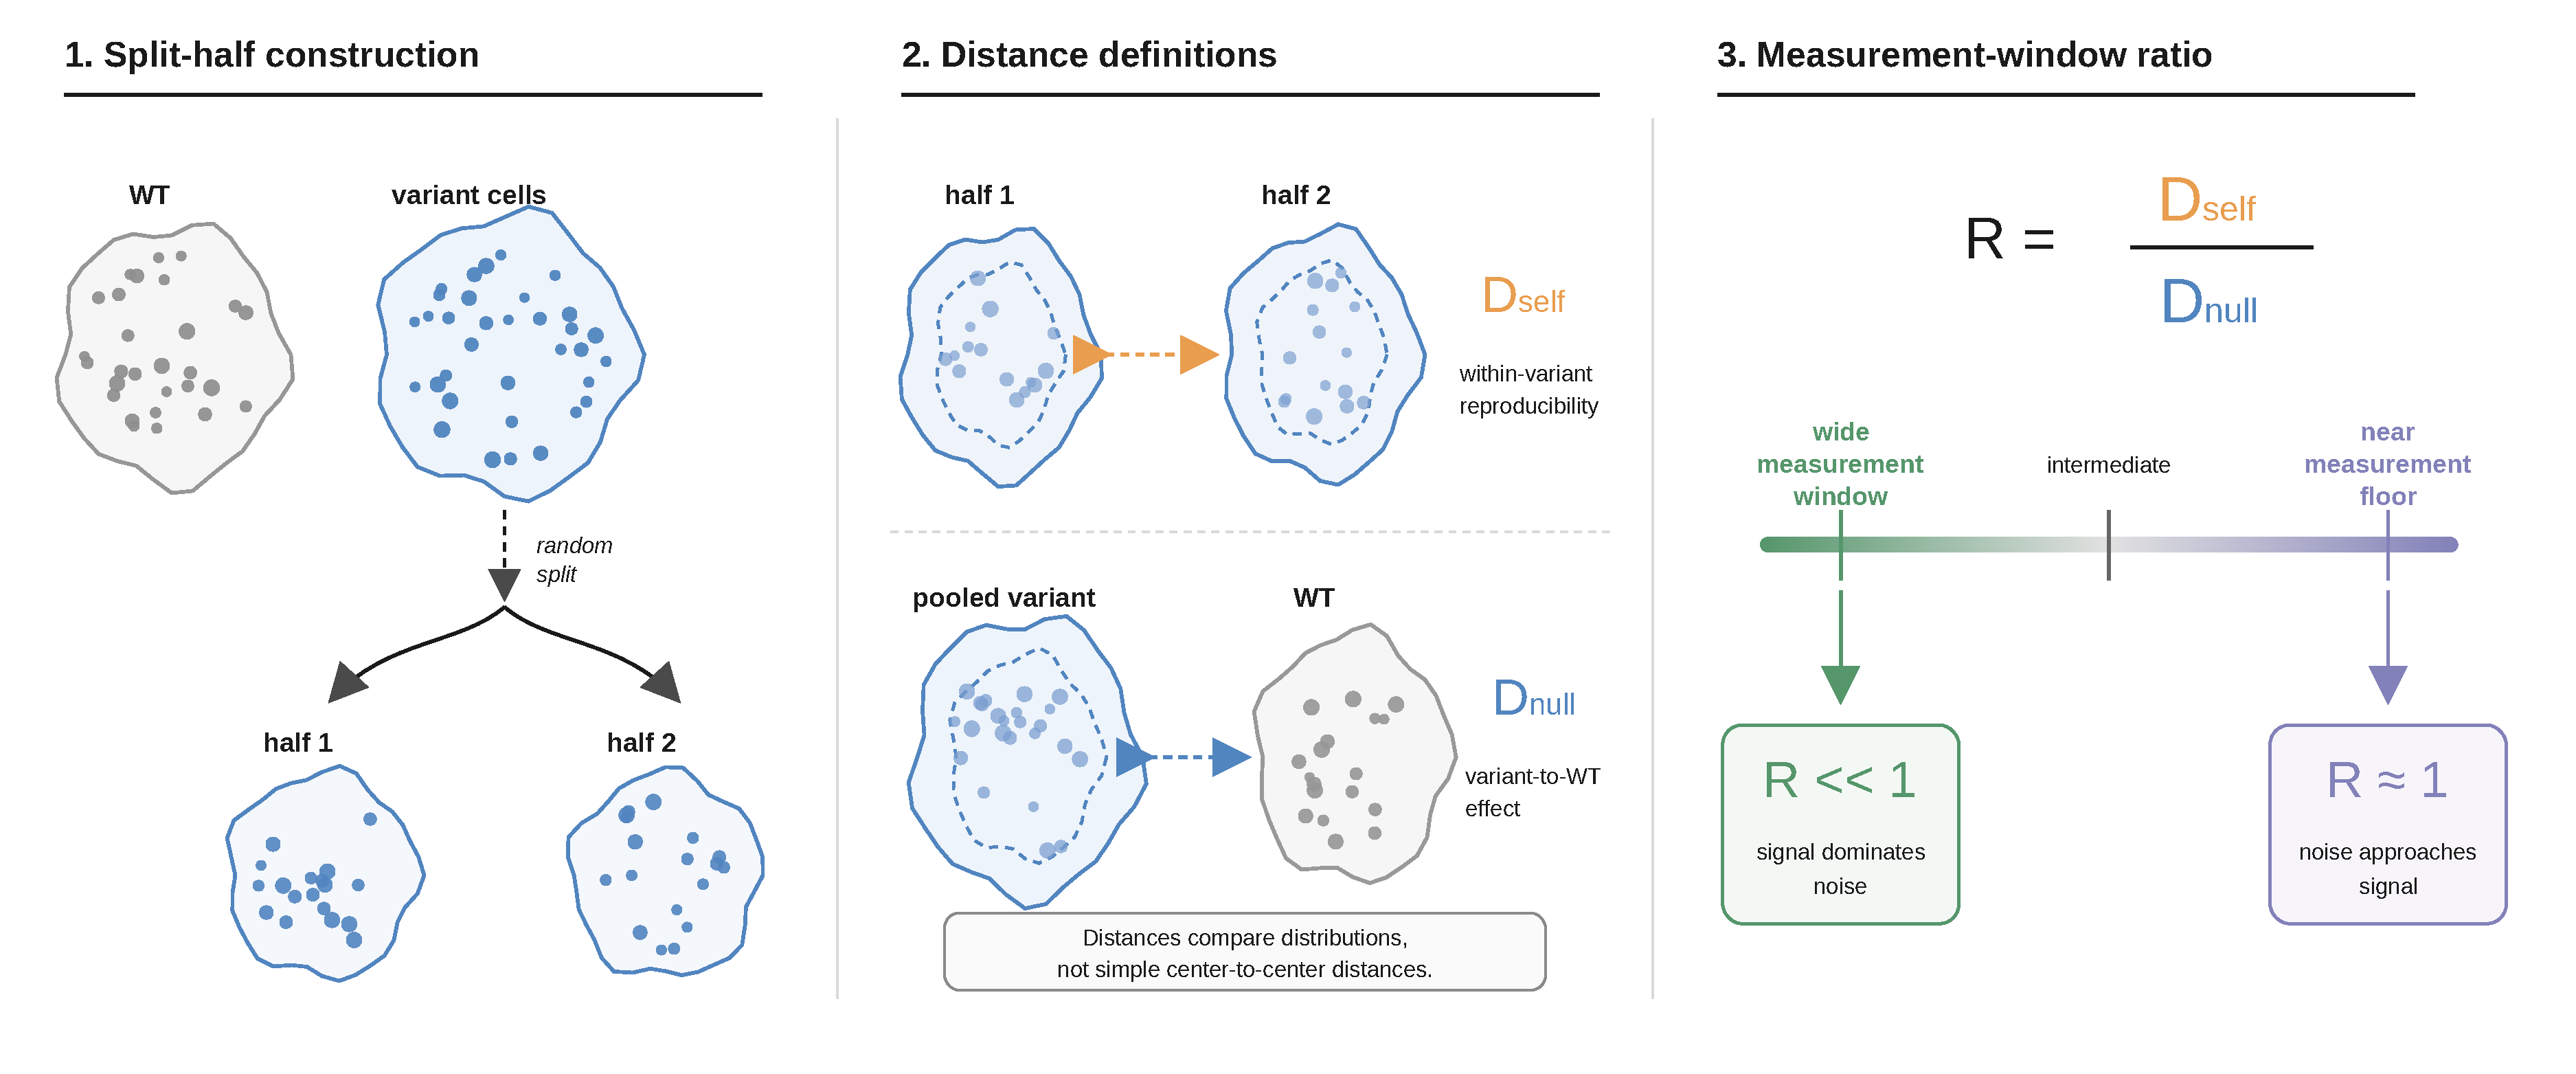
\includegraphics[width=46mm]{Fig3a.pdf}};
  \node[anchor=north west,inner sep=0] at (54,164) {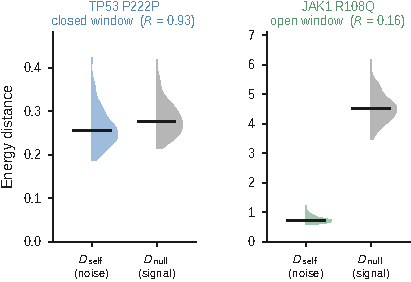
\includegraphics[width=60mm]{fig3b_windows.pdf}};
  \node[anchor=north west,inner sep=0] at (118,163){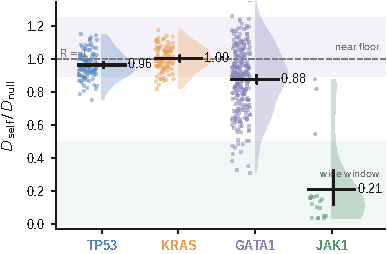
\includegraphics[width=64mm]{fig3c_ratio.pdf}};
  % row 2: d sibling-pair resolvable | e classifier (identification)
  \node[anchor=north west,inner sep=0] at (10,114) {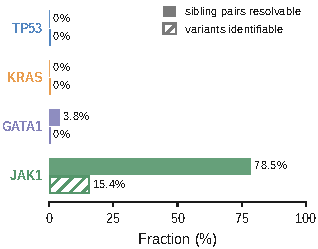
\includegraphics[width=74mm]{fig3g_detect_ident.pdf}};
  \node[anchor=north west,inner sep=0] at (96,114) {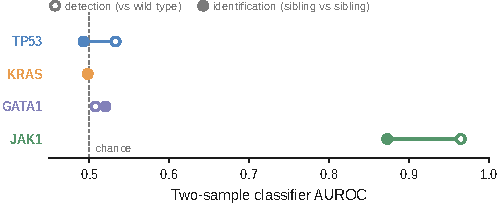
\includegraphics[width=76mm]{fig3h_classifier.pdf}};
  % row 3: f landscape | g titration | h rankable (determinants)
  \node[anchor=north west,inner sep=0] at (4,50)  {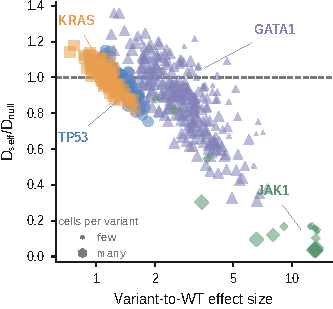
\includegraphics[width=54mm]{fig3d_landscape.pdf}};
  \node[anchor=north west,inner sep=0] at (62,50) {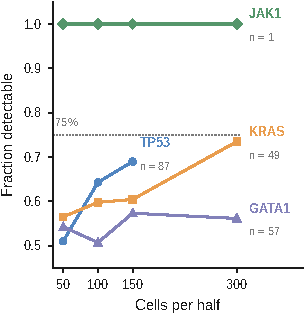
\includegraphics[width=52mm]{fig3e_titration.pdf}};
  \node[anchor=north west,inner sep=0] at (120,50){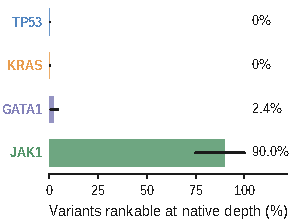
\includegraphics[width=58mm]{fig3f_rankable.pdf}};
  % panel letters
  \tikzset{plab/.style={font=\bfseries\large,anchor=north west,inner sep=0}}
  \node[plab] at (1,166) {a};   \node[plab] at (51,166) {b};   \node[plab] at (115,166) {c};
  \node[plab] at (7,116) {d};   \node[plab] at (93,116) {e};
  \node[plab] at (1,52) {f};    \node[plab] at (59,52) {g};    \node[plab] at (117,52) {h};
\end{tikzpicture}
\end{document}
